\documentclass{article}

% Essential packages
\usepackage{graphicx}   % For image handling
\usepackage{subcaption} % For multi images
\usepackage{caption}    % For proper captions
\usepackage{listings}   % For code listings
\usepackage{fontspec}   % For custom fonts
\usepackage{xcolor}     % For color support
\usepackage{tcolorbox}  % For code block boxes
\usepackage{etoolbox}   % For patching and command manipulation
\usepackage{titlesec}   % For section formatting
\usepackage{parskip}    % For customisable paragraph formating
\usepackage{comment}    % For being able to comment out sections
\usepackage{geometry}   % For managing page size and margins
\usepackage{hyperref}   % For embedding links, like URL's
\usepackage{bigstrut}
\usepackage{multirow}
\usepackage{colortbl}
\usepackage{amsmath}    % For math and equation formatting

\tcbuselibrary{listings, skins, breakable}  %Librarary to make code blocks multipage


%   ############################## Customisation ##############################

% Document metadata
\title{\fontsize{24}{36}\selectfont Programable Logic Circuts\\ %Edit title here \\ means new line
Lab 03} % Line 2 of title, its not subtitle, that is possible to, google it
\author{Sølve Kjelseth} % Input your name
\date{\today} % Auto updates the date, untill you export it, replace with hardcoded date if you need

% Adjust the body text font size to 12pt without affecting section headings
\renewcommand{\normalsize}{\fontsize{12}{16}\selectfont}

% Adjust the paragraph spacing, either as indentation or/and line spaceing
\setlength{\parindent}{0pt}  % Remove indentation
\setlength{\parskip}{6pt}    % Add vertical space between paragraphs

% Customisation of fonts and colors
\setmainfont{Times New Roman}
\setmonofont{JetBrains Mono}
\definecolor{background}{RGB}{225, 219, 202}
\definecolor{darkAccent}{RGB}{140, 98, 64}
\definecolor{commentGreen}{RGB}{26, 159, 32}
\definecolor{keywordPurple}{RGB}{229, 24, 192}
\definecolor{keywordBlue}{RGB}{5, 142, 217}
\definecolor{portOrange}{RGB}{234, 72, 31}
\definecolor{darkGray}{RGB}{60, 60, 60}

% Link color customization
\hypersetup{
    colorlinks=true,
    linkcolor=darkGray, % Internal links such as table of contents or figure referencing
    urlcolor=keywordBlue % URL colors
    }
\urlstyle{same} % Makes url in the same style as the rest of the document

% Customisation of margins and paper size
\geometry{
 a4paper,
 left = 30mm,
 right = 30mm,
 top = 30mm,
 bottom = 30mm
 }

% Sections formatting and numbering
% Sets the font to monospace for section, subsection and subsubsection
% and sets the format to be numbers with . between and at the end
\renewcommand{\thesection}{\texttt{\arabic{section}.}}
\renewcommand{\thesubsection}{\texttt{\arabic{section}.\arabic{subsection}.}}
\renewcommand{\thesubsubsection}{\texttt{\arabic{section}.\arabic{subsection}.\arabic{subsubsection}.}}

\setcounter{section}{-1}  % Start section numbering from 0, delete this to start from 1


\newcounter{codeblock} % Define new counter
\renewcommand{\thecodeblock}{\arabic{section}.\arabic{codeblock}} % Define numbering format

% Makes section monospace font and start each subsection from 0 and figure number
\let\oldsection\section
\renewcommand{\section}[1]{%
  \oldsection{\texttt{#1}} % Make section title monospace
  \setcounter{subsection}{-1} % Makes subsection start from 0, delete this line to start from 1
  \setcounter{figure}{-1} % Makes figure numbers start from 0, delete this line to start from 1
  \setcounter{table}{-1} % Makes table numbers start from 0, delete this line to start from 1
  \setcounter{codeblock}{-1}
}


% Makes subsection monospace font and start each subsubsection from 0
\let\oldsubsection\subsection
\renewcommand{\subsection}[1]{%
  \oldsubsection{\texttt{#1}}% Make subsection title monospace
  \setcounter{subsubsection}{-1}% Makes subsubsection start from 0, delete this line to start from 1
}

% Makes subsubsection monospace font
\let\oldsubsubsection\subsubsection
\renewcommand{\subsubsection}[1]{%
  \oldsubsubsection{\texttt{#1}}% Make subsubsection title monospace
}

% Makes every new section start on a new page, except for the first section, section 0
\pretocmd{\section}{%
  \ifnum\value{section}=-1 \else\clearpage\fi % Replace -1 with 0 if sections start at nr. 1
}{}{}

% Makes Table of contents a subsection
\makeatletter
\renewcommand{\tableofcontents}{%
    \subsection{Table of Contents} % Numbered subsection named Table of contents
    \@starttoc{toc}%
}
\makeatother

% Makes List of figures a subsection
\makeatletter
\renewcommand{\listoffigures}{%
    \subsection{List of Figures} % Numbered subsection named List of figures
    \@starttoc{lof}%
}
\makeatother

% Makes List of tables a subsection
\makeatletter
\renewcommand{\listoftables}{%
    \subsection{List of Tables} % Numbered subsection named List of tables
    \@starttoc{lot}%
}
\makeatother


% Makes every figure be formated as section number.figure number
\renewcommand{\thefigure}{\arabic{section}.\arabic{figure}}

% Makes every table be formated as section number.table number
\renewcommand{\thetable}{\arabic{section}.\arabic{table}}
\AtBeginEnvironment{tabular}{\ttfamily} % Monozpaced font within tables

% Add keywords to be highlited in blue below. Note that all reserved
% keywords from VHDL is already in purple and should not be added here
% too as duplicates will cause issues. Therfore compile this document
% after pasting in code and only add non-highlited words to this list.
% Also, there is not a list for orange keywords, used for ports here.
\lstdefinelanguage{VHDL+}{
    language     = VHDL,
    morestring = [b]',
    morekeywords = [2]{
        IEEE,
        std_logic_1164, std_logic, std_logic_vector},
    morekeywords = [3]{
        SW, LEDR, KEY,
        HEX0, HEX1, HEX2, HEX3, HEX4, HEX5, HEX6},
    sensitive = false
}


%   ############################## Advanced customisation ##############################

% Customisation of list style inside code block
\lstdefinestyle{VHDL}{
    language = VHDL+, % Uses the extra higlights from above
    % The folloowing lines defines color for highlighting, other changes like
    % italic, bold or different fonts can also be added to this
    escapechar = §,
    commentstyle = \color{commentGreen}, 
    keywordstyle = \color{keywordPurple},
    keywordstyle = [2]\color{keywordBlue},
    keywordstyle = [3]\color{portOrange},
    stringstyle = \color{darkAccent},
    basicstyle = \ttfamily\small, % Default font inside code block
    numberstyle = \ttfamily\color{darkAccent}, % Style of line numbering
    numbers = left, % Line numbering on left side
    breakatwhitespace = false, % Don't start new line with only whitspaces
    breaklines = true, % If line is to long it will wrap to next line (line number does not increase)
    keepspaces = true, % Indents works logical
    showspaces = false, % Space is blank character, set to true to show dots instad
    showstringspaces = false, % Same as above but inside strings
    showtabs = false, % Tab is also blank character, set to true to show dashes
    tabsize = 4, % Tabsize is set to 4, this works well with code from notepad++
    % Dont mess with the ones below unless you want to mess with the box as well
    % These took some time to line up such that it looks natural
    numbersep = 10pt, % Adjust distance between numbers and code
    xleftmargin = -8pt,% Negative margin to pull code text closer to the left border
}

% This is for code where VHDL is not an argument
\lstdefinestyle{Example Code}{
    basicstyle = \ttfamily\small, % Default font inside code block
    numberstyle = \ttfamily\color{darkAccent}, % Style of line numbering
    numbers = left, % Line numbering on left side
    breakatwhitespace = false, % Don't start new line with only whitspaces
    breaklines = true, % If line is to long it will wrap to next line (line number does not increase)
    keepspaces = true, % Indents works logical
    showspaces = false, % Space is blank character, set to true to show dots instad
    showstringspaces = false, % Same as above but inside strings
    showtabs = false, % Tab is also blank character, set to true to show dashes
    tabsize = 4, % Tabsize is set to 4, this works well with code from notepad++
    % Dont mess with the ones below unless you want to mess with the box as well
    % These took some time to line up such that it looks natural
    numbersep = 10pt, % Adjust distance between numbers and code
    xleftmargin = -8pt,% Negative margin to pull code text closer to the left border
}

\lstset{style = Example Code} %Sets the default style to Example Code

% Customisation of code block itself
\newtcolorbox[auto counter, number within=section]{codeBlock}[2][]{
    colback=background, % Background color for the code block
    colframe=darkAccent, % Border color for the code block
    listing only, %Makes it contain the listing
    arc=10pt, % Rounded corners size
    sharp corners=northeast, % Make top-right corner sharp for the main box
    enhanced jigsaw, % Essential dont mess with it
    breakable, % Allows content to be multipage
    top=-4pt, % Made to line up text dont mess with it
    bottom=-4pt, % Same as above
    before skip=0pt, after skip=10pt, % Adjust spacing before and after the box
    boxrule=1pt, % Border thickness of the main box
    overlay unbroken and first={\node[ % Create label box in the top-right corner
        anchor=north east,      %Position of box, same as sharp corner in this case
        fill=background,        %Background color same as main box
        draw=darkAccent,        %Outline color, same as main box
        line width=1pt,         %Outline thickness, same as main box
        text=keywordPurple,     %Text color
        font=\ttfamily,         %Text font and size
        inner sep=6pt,          %Spacing inside
        minimum width=16pt,     %Minimum box with, it autoresizes depending on text
        minimum height=12pt,    %Minimum box height, it autoresizes depending on text
        text centered,          %Centres the text with the spacing
        sharp corners]          %Makes corners sharp
        at ([xshift=0pt, yshift=0pt]frame.north east) % Position, aligned with corner on main box
        {#2}; % Types your argument in the top corner as a label
    }
}

\newcommand{\writecode}[3][Example Code]{%
    \par\medskip % Adds some vertical spacing before the caption
    \refstepcounter{codeblock} % Step the figure counter
    \label{Code:#2} % Unique label for referencing
    \begin{center} % Center the caption
        Code \thecodeblock: #3 % Fake caption
    \end{center}
    \addcontentsline{lof}{figure}{Code \thecodeblock: #3} % Manually add entry to List of Figures
    \par\medskip % Adds some vertical spacing after the caption before the code block
    \begin{codeBlock}{#1}% arg 1 (default Example Code) will be written in the top right corner box
        \lstinputlisting[style=#1]{Code/#2}% arg 1 style is used and arg 2 is filename
    \end{codeBlock}%
    \par\medskip % Adds some vertical spacing after the code block
}




\newcommand{\figcaption}[1]{%
    \caption[]{#1} % Suppress the default entry in LoF
    \addcontentsline{lof}{figure}{Figure \thefigure: #1} % Manually add the correct format
}

\newcommand{\tabcaption}[1]{%
    \caption[]{#1} % Suppress the default entry in LoT
    \addcontentsline{lot}{table}{Table \thetable: #1} % Manually add the correct format
}

\newcommand{\unit}[1]{\ensuremath{\, \mathrm{#1}}}



%   ############################## Document begins here ##############################
\begin{document}

\maketitle % Makes title front page based on the title, author and date metadata, change at the top


%   ############################## Section ##############################
\addtocontents{toc}{\protect\setcounter{tocdepth}{0}} % Temporarily hide from TOC
\section{Introduction} % Numbered section named Introduction
This is the third report in this course, detailing the completion of the third lab exercise. With the purpose is to investigate latches, flip-flops, and registers.\par
Note: The VHDL and \LaTeX\ code is open source
\href{https://github.com/Kjelseth/PLK_lab.git}{github link}.
\clearpage
\tableofcontents % Generate TOC
\clearpage
\listoffigures % List of figures
\clearpage
\listoftables % List of tables
\addtocontents{toc}{\protect\setcounter{tocdepth}{2}} % Restore TOC depth


%   ############################## Section ##############################
\section{Part 1}
The purpose of this task was to examine the structure of the code, both to see how it was synthesized and also to simulate it to see if it was working.

\subsection{Code}
\writecode[VHDL]{Part1_TLE.vhd}{Code with equal function to the one included in the task}

\clearpage
\subsection{RTL}
The synthesization of the VHDL code is shown in figure~\ref{fig:p1_RTL}. It looks logically equal to the schematic provided by the task.

\begin{figure}[h]
    \centering
    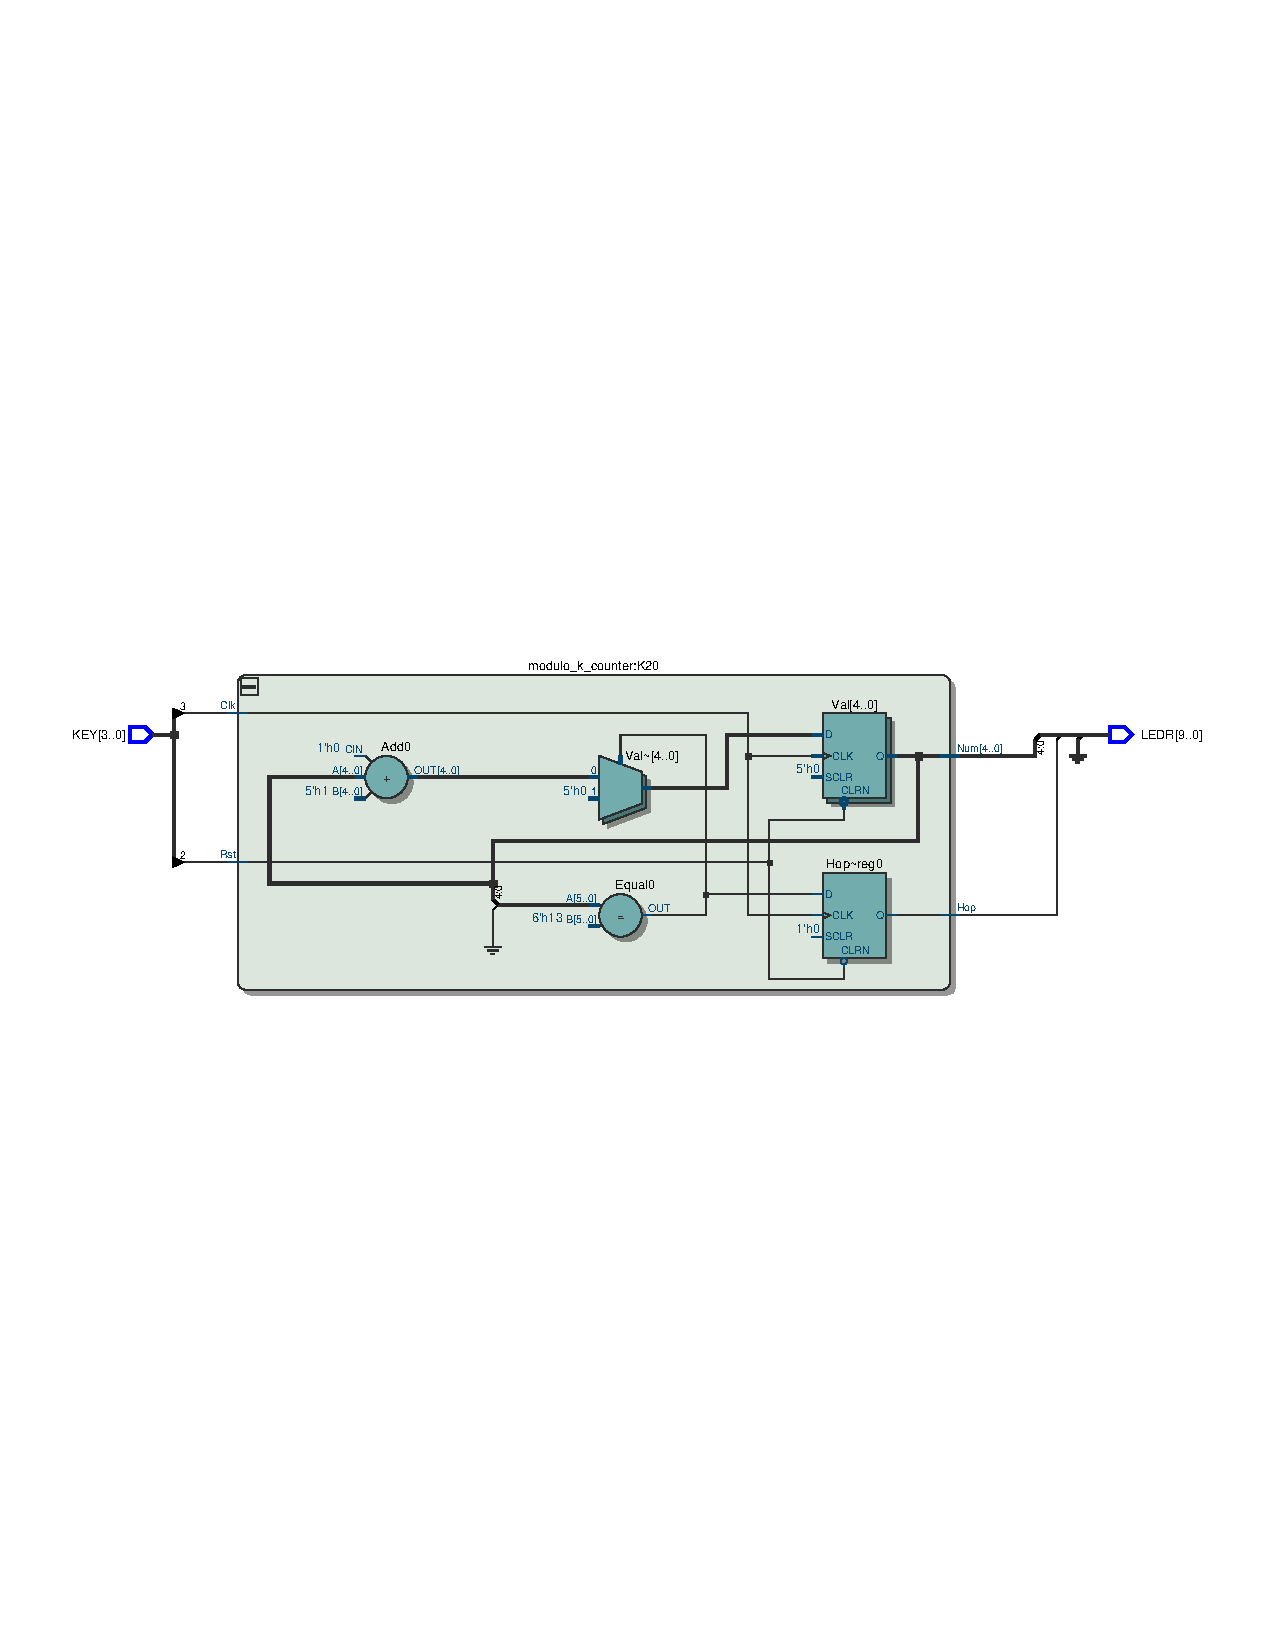
\includegraphics[width=1\textwidth]{Figures/Part1_RTL.jpg}
    \figcaption{RTL for the TLE}
    \label{fig:p1_RTL}
\end{figure}

\subsection{Results}
Doing a simulation using Quartus, the resulting output is as expected. Simulation both \(R\) and \(S\) to be on at the same time resulted in some out of bounds calculating and the simulation timing out. Needless to say it does not really make sense to have such an input anyway and therefore is omitted. Output is as expected.

\begin{figure}[h]
    \centering
    \includegraphics[width=1\textwidth]{Figures/Part1_sim.jpg}
    \figcaption{Simulation results}
    \label{fig:p1_sim}
\end{figure}


%   ############################## Section ##############################
\section{Part 2}
The purpose of this task was to first make a D-latch and then make another project that implemented it as an instance of a component and testing it on the board.

Note: For the first part only, the standalone D-latch, I made a mistake when restructuring the code for readability. Looking at code~\ref{Code:Part2_1_TLE.vhd} at line 18 and 19. Here \verb|R_g| and \verb|S_g| should be swapped. This makes the circuit equivalent to either having swapped inputs or inverted the output.

\subsection{Code}
\writecode[VHDL]{Part2_1_TLE.vhd}{Simple D-latch with a small I/O mistake}
Now to implement this as a component, the TLE was first made. Import of such a component and mapping it to the inputs and outputs used by the FPGA was done in the TLE. Then the code~\ref{Code:Part2_1_TLE.vhd} was copied over to code~\ref{Code:Part2_2_and_3_Dl.vhd}, a more general VHDL file where I/O is not tied to the FPGA board. This was done before the error noted above and therefore will not follow through more tasks.

\clearpage
\writecode[VHDL]{Part2_2_TLE.vhd}{TLE importing a D-latch}
\writecode[VHDL]{Part2_2_and_3_Dl.vhd}{General D-latch component}

\clearpage
\subsection{RTL}
RTL of the first D-latch with the I/O mistake is omitted as there is no value in adding it to the report, when the general D-latch shown in the expanded RTL in figure~\ref{fig:p2_RTL_Dl} is the same without the error.
\begin{figure}[h]
    \centering
    \includegraphics[width=1\textwidth]{Figures/Part2b_RTL.jpg}
    \figcaption{TLE with a D-latch component}
    \label{fig:p2_RTL_TLE}
\end{figure}
\begin{figure}[h]
    \centering
    \includegraphics[width=1\textwidth]{Figures/Part2b_RTL_Expanded.jpg}
    \figcaption{The D-latch component expanded}
    \label{fig:p2_RTL_Dl}
\end{figure}

\subsection{Results}
The first part was simulated, here you can see that the input/output is reversed to what it should have been.
\begin{figure}[h]
    \centering
    \includegraphics[width=1\textwidth]{Figures/Part2a_sim.jpg}
    \figcaption{Simulation of the first D-latch with the I/O mistake}
    \label{fig:p2_sim}
\end{figure}
Implementing the second part code on the FPGA the results was as expected. Here it is clear that when \verb|Clk| is high, \verb|D| is continuously overwriting the output LED and when \verb|Clk| is low, the output is equal to the last saved state of \verb|D|.

\clearpage
\begin{figure}[h]
    \centering
    \begin{subfigure}[t]{0.45\textwidth}
        \centering
        \includegraphics[width=1\textwidth]{Figures/Part2b_1.jpg}
        \caption{Clk low, D high not registered}
        \label{fig:p2b_1}
    \end{subfigure}
    \hfill
    \begin{subfigure}[t]{0.45\textwidth}
        \centering
        \includegraphics[width=1\textwidth]{Figures/Part2b_2.jpg}
        \caption{Clk low, D low already stored}
        \label{fig:p2b_2}
    \end{subfigure}
    
    \begin{subfigure}[t]{0.45\textwidth}
        \centering
        \includegraphics[width=1\textwidth]{Figures/Part2b_3.jpg}
        \caption{Clk high, D low already stored}
        \label{fig:p2b_3}
    \end{subfigure}
    \hfill
    \begin{subfigure}[t]{0.45\textwidth}
        \centering
        \includegraphics[width=1\textwidth]{Figures/Part2b_4.jpg}
        \caption{Clk high, D high registered}
        \label{fig:p2b_4}
    \end{subfigure}
    
    \begin{subfigure}[t]{0.45\textwidth}
        \centering
        \includegraphics[width=1\textwidth]{Figures/Part2b_5.jpg}
        \caption{Clk low, D high already stored}
        \label{fig:p2b_5}
    \end{subfigure}
    \hfill
    \begin{subfigure}[t]{0.45\textwidth}
        \centering
        \includegraphics[width=1\textwidth]{Figures/Part2b_6.jpg}
        \caption{Clk low, D low not registered}
        \label{fig:p2b_6}
    \end{subfigure}
    \figcaption{D-latch on the FPGA using a component works as expected}
    \label{fig:p2_results}
\end{figure}

%   ############################## Section ##############################
\section{Part 3}
The purpose of this task was to continue last part and instead of a single instance of a D-latch, use two instances, to make a D-flip-flop.

\subsection{Code}
\writecode[VHDL]{Part3_TLE.vhd}{TLE using two instances of a D-latch}
The D-latch component used here is code~\ref{Code:Part2_2_and_3_Dl.vhd}.


\subsection{RTL}
\begin{figure}[h]
    \centering
    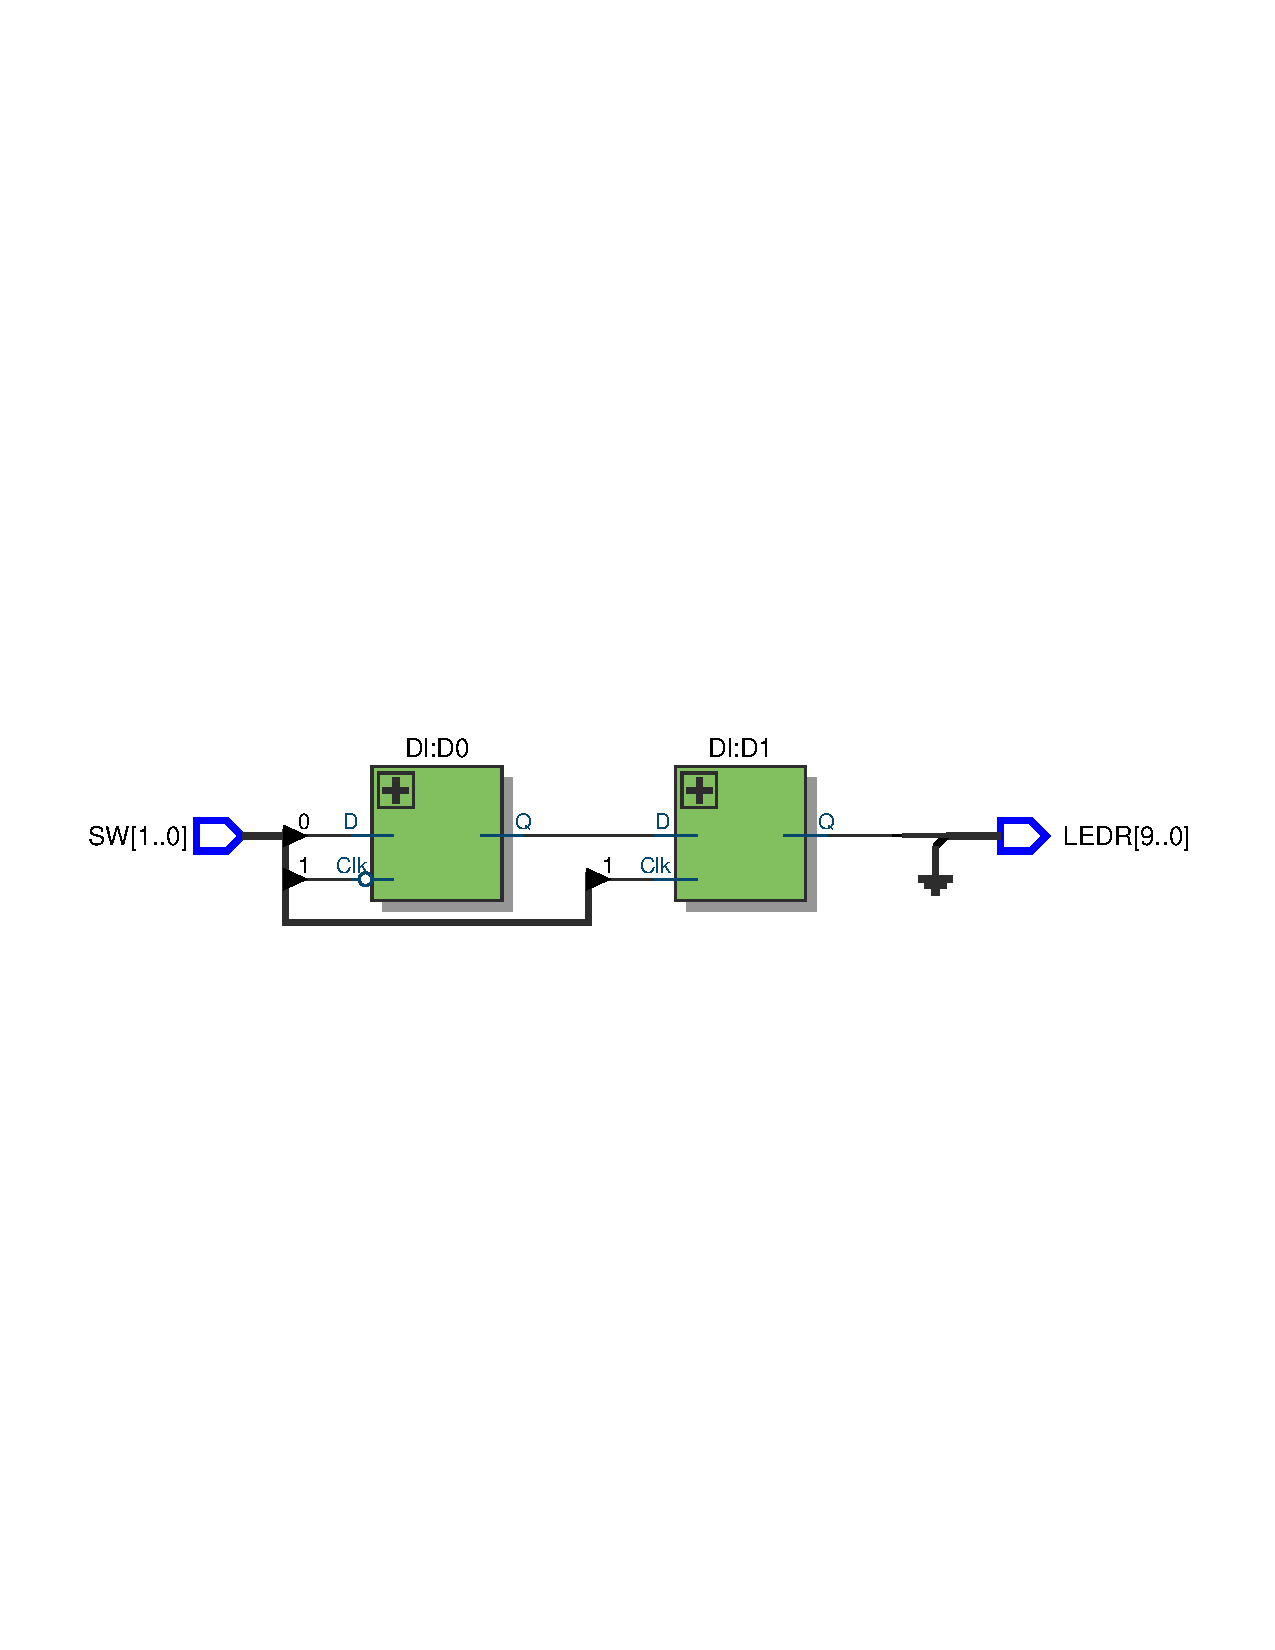
\includegraphics[width=1\textwidth]{Figures/Part3_RTL.jpg}
    \figcaption{RTL of the TLE with two instances}
    \label{fig:p3_RTL}
\end{figure}

\subsection{Results}
Implementing the code on the FPGA the results was as expected. Here it is clear that when \verb|Clk| has a rising edge, \verb|D| is saved to the output LED and when \verb|Clk| is high or low, the output is equal to the last saved state of \verb|D|.
\clearpage
\begin{figure}[h]
    \centering
    \begin{subfigure}[t]{0.45\textwidth}
        \centering
        \includegraphics[width=1\textwidth]{Figures/Part3_1.jpg}
        \caption{Clk low, D low already stored}
        \label{fig:p3_1}
    \end{subfigure}
    \hfill
    \begin{subfigure}[t]{0.45\textwidth}
        \centering
        \includegraphics[width=1\textwidth]{Figures/Part3_2.jpg}
        \caption{Clk low, D high not registered}
        \label{fig:p3_2}
    \end{subfigure}
    
    \begin{subfigure}[t]{0.45\textwidth}
        \centering
        \includegraphics[width=1\textwidth]{Figures/Part3_3.jpg}
        \caption{Clk high, D high registered}
        \label{fig:p3_3}
    \end{subfigure}
    \hfill
    \begin{subfigure}[t]{0.45\textwidth}
        \centering
        \includegraphics[width=1\textwidth]{Figures/Part3_4.jpg}
        \caption{Clk high, D low not registered}
        \label{fig:p3_4}
    \end{subfigure}
    
    \begin{subfigure}[t]{0.45\textwidth}
        \centering
        \includegraphics[width=1\textwidth]{Figures/Part3_5.jpg}
        \caption{Clk low, D low not registered}
        \label{fig:p3_5}
    \end{subfigure}
    \hfill
    \begin{subfigure}[t]{0.45\textwidth}
        \centering
        \includegraphics[width=1\textwidth]{Figures/Part3_6.jpg}
        \caption{Clk high, D low registered}
        \label{fig:p3_6}
    \end{subfigure}
    \figcaption{D-flip-flop on the FPGA using two D-latches works as expected}
    \label{fig:p3_results}
\end{figure}


%   ############################## Section ##############################
\section{Part 4}
The purpose of this task was to use behavioural code to implement a D-latch and a D-flip-flop. Then to see how the different data outputs are stored between a D-latch, a positive edge D-flip-flop and a negative edge D-flip-flop.

\subsection{Code}
\writecode[VHDL]{Part4_TLE.vhd}{TLE of a circuit to compare different data storage}

\clearpage
The D-latch code was already provided by the task, and instead of doing both a rising and a falling edge trigger separate for the D-flip-flops a common component was made and the \verb|Clk| input inverted for the second instance.
\writecode[VHDL]{Part4_Dl.vhd}{Code with equal function to the one included in the task}
\writecode[VHDL]{Part4_Dff.vhd}{Behavioural code for a D-flip-flop}

\clearpage
\subsection{RTL}
\begin{figure}[h]
    \centering
    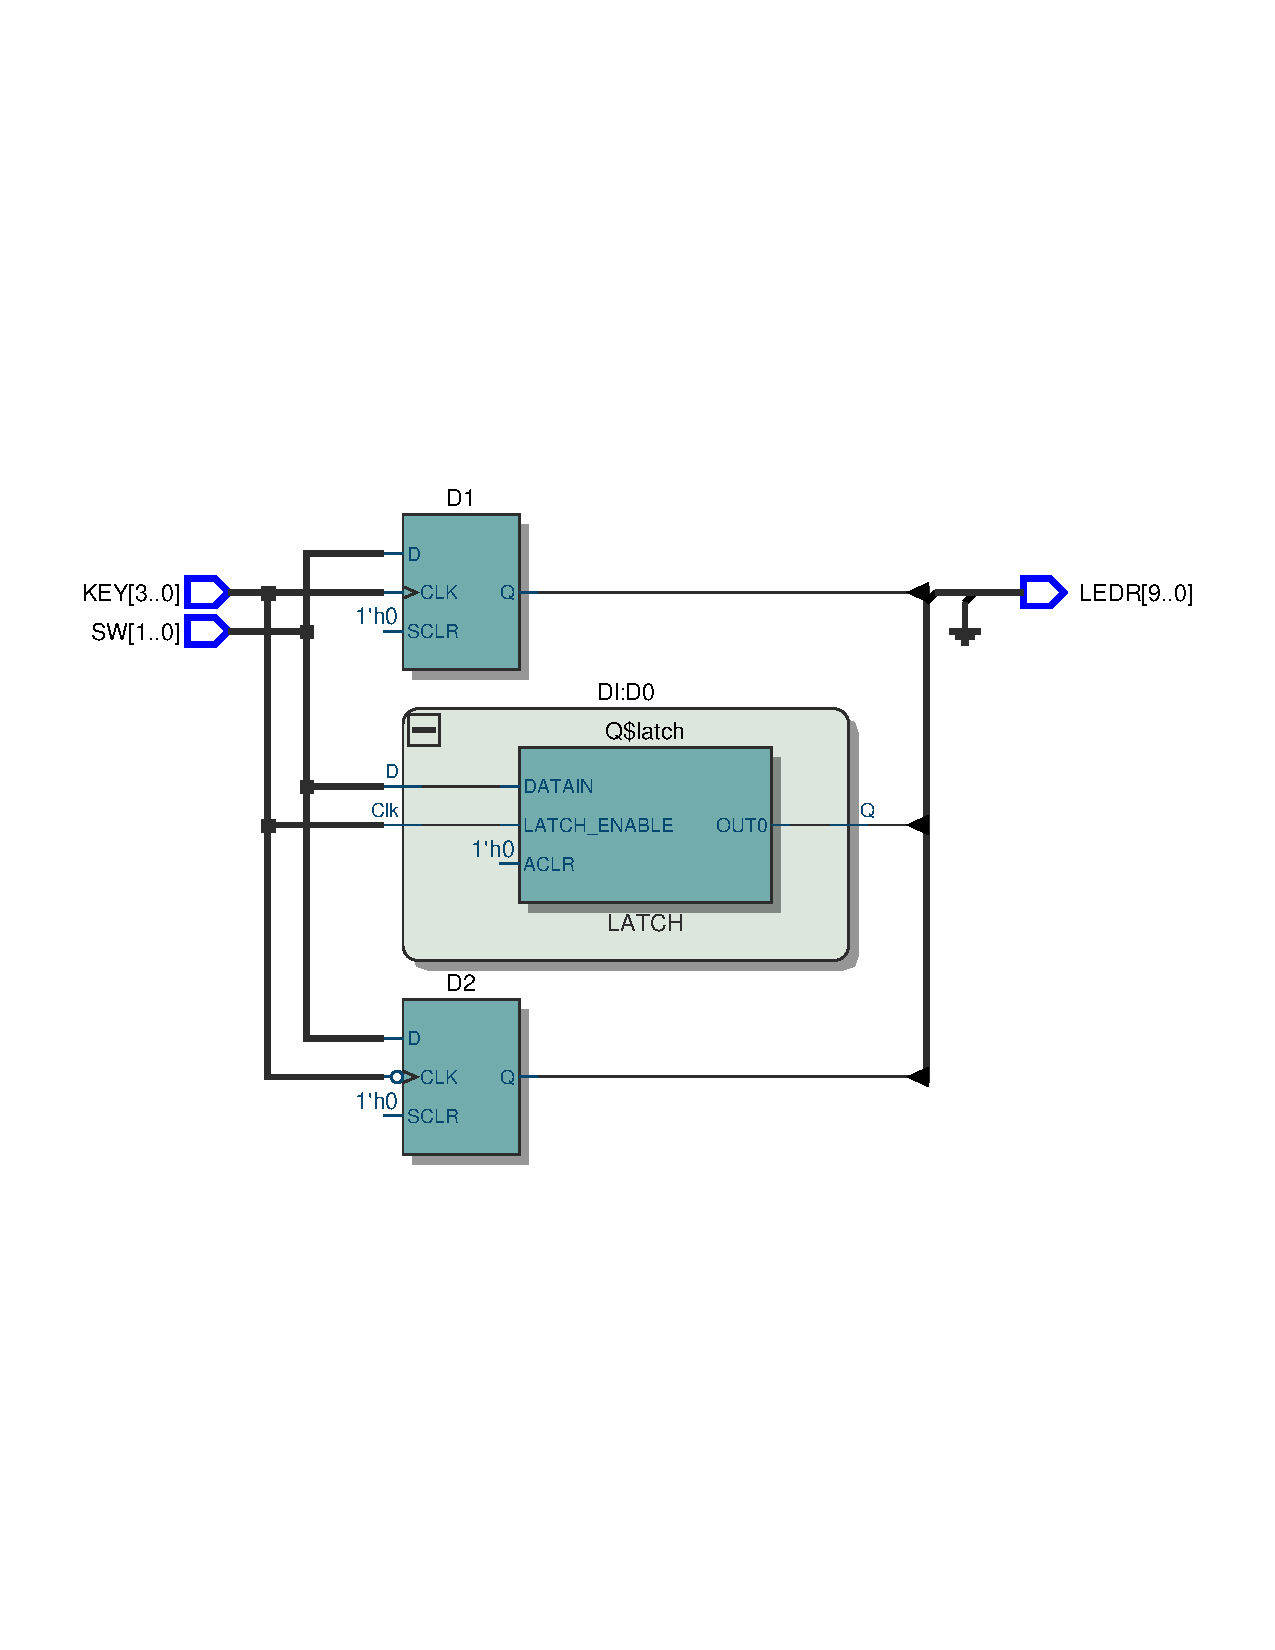
\includegraphics[width=1\textwidth]{Figures/Part4_RTL.jpg}
    \figcaption{RTL of the TLE with all three instances}
    \label{fig:p4_RTL}
\end{figure}

\subsection{Results}
Implementing the code on the FPGA the results was as expected. The output is shown as the following: In \textcolor{red}{red}, the negative edge D-flip-flop, in \textcolor{green}{green} the positive edge D-flip flop and in \textcolor{blue}{blue}, the D-latch. It is also worth noting that the button \verb|Clk| is connected to is pull-up, as it is normally high.\par
Observations shows that when \verb|Clk| is high, unpressed, the, \verb|D| is continuously controlling the \textcolor{blue}{blue output}, and the others are unaffected. While depressing the button, giving a falling edge to \verb|Clk|, the state of \verb|D| is saved to the \textcolor{red}{red output}. When letting go of the button, giving a rising edge to \verb|Clk|, the state of \verb|D| is stored in the \textcolor{green}{green output}, as expected.

\clearpage
\begin{figure}[h]
    \centering
    \begin{subfigure}[t]{0.45\textwidth}
        \centering
        \includegraphics[width=1\textwidth]{Figures/Part4_1.jpg}
        \caption{D low, Clk high}
        \label{fig:p4_1}
    \end{subfigure}
    \hfill
    \begin{subfigure}[t]{0.45\textwidth}
        \centering
        \includegraphics[width=1\textwidth]{Figures/Part4_2.jpg}
        \caption{D high, Clk high}
        \label{fig:p4_2}
    \end{subfigure}
    
    \begin{subfigure}[t]{0.45\textwidth}
        \centering
        \includegraphics[width=1\textwidth]{Figures/Part4_3.jpg}
        \caption{D high, Clk low(falling)}
        \label{fig:p4_3}
    \end{subfigure}
    \hfill
    \begin{subfigure}[t]{0.45\textwidth}
        \centering
        \includegraphics[width=1\textwidth]{Figures/Part4_4.jpg}
        \caption{D high, Clk high(rising)}
        \label{fig:p4_4}
    \end{subfigure}
    
    \begin{subfigure}[t]{0.45\textwidth}
        \centering
        \includegraphics[width=1\textwidth]{Figures/Part4_5.jpg}
        \caption{D low, Clk high}
        \label{fig:p4_5}
    \end{subfigure}
    \hfill
    \begin{subfigure}[t]{0.45\textwidth}
        \centering
        \includegraphics[width=1\textwidth]{Figures/Part4_6.jpg}
        \caption{D low, Clk low(falling)}
        \label{fig:p4_6}
    \end{subfigure}
    \figcaption{D-flip-flop and D-latches}
    \label{fig:p4_results}
\end{figure}


%   ############################## Section ##############################
\section{Part 5}

The purpose of this task was to use a register to store a value, and combine with knowledge from previous lab exercises to integrate an adder, and some 7-segment displays.

\subsection{Solving}
The starting point was making a decoder for the 7-segment displays, the task specified to operate in hexadecimal. That made it much simpler as instead of needing a BCD converter or similar, the 4 most significant bits could control the most significant digit and the 4 least significant bits could control the least significant digit, completely independently. Using figure~\ref{fig:7seg} table~\ref{tab:decoder} was made for use in the decoder.\par


\begin{figure}[h]
    \centering
    \includegraphics[width=0.4\textwidth]{Figures/7seg.jpg}
    \figcaption{7 segment FPGA bit order}
    \label{fig:7seg}
\end{figure}

\clearpage

% Table generated by Excel2LaTeX from sheet 'Part5'
\begin{table}[htbp]
  \centering
  \caption{Output values for decoder based on input}
    \begin{tabular}{|c|c|c|c|c|c|c|c|c|c|c|c|c|}
    \hline
    \multirow{2}[4]{*}{NR} & \multicolumn{4}{c|}{Num}      & \multicolumn{7}{c|}{HEX}                              & String \bigstrut\\
\cline{2-13}          & 3     & 2     & 1     & 0     & 6     & 5     & 4     & 3     & 2     & 1     & 0     & "6543210" \bigstrut\\
    \hline
    0     & \cellcolor[rgb]{ .851,  .851,  .851}0 & \cellcolor[rgb]{ .851,  .851,  .851}0 & \cellcolor[rgb]{ .851,  .851,  .851}0 & \cellcolor[rgb]{ .851,  .851,  .851}0 & \cellcolor[rgb]{ .71,  .902,  .635}1 & \cellcolor[rgb]{ .71,  .902,  .635}0 & \cellcolor[rgb]{ .71,  .902,  .635}0 & \cellcolor[rgb]{ .71,  .902,  .635}0 & \cellcolor[rgb]{ .71,  .902,  .635}0 & \cellcolor[rgb]{ .71,  .902,  .635}0 & \cellcolor[rgb]{ .71,  .902,  .635}0 & \cellcolor[rgb]{ .58,  .863,  .973}"1000000" \bigstrut\\
    \hline
    1     & \cellcolor[rgb]{ .851,  .851,  .851}0 & \cellcolor[rgb]{ .851,  .851,  .851}0 & \cellcolor[rgb]{ .851,  .851,  .851}0 & \cellcolor[rgb]{ .851,  .851,  .851}1 & \cellcolor[rgb]{ .71,  .902,  .635}1 & \cellcolor[rgb]{ .71,  .902,  .635}1 & \cellcolor[rgb]{ .71,  .902,  .635}1 & \cellcolor[rgb]{ .71,  .902,  .635}1 & \cellcolor[rgb]{ .71,  .902,  .635}0 & \cellcolor[rgb]{ .71,  .902,  .635}0 & \cellcolor[rgb]{ .71,  .902,  .635}1 & \cellcolor[rgb]{ .58,  .863,  .973}"1111001" \bigstrut\\
    \hline
    2     & \cellcolor[rgb]{ .851,  .851,  .851}0 & \cellcolor[rgb]{ .851,  .851,  .851}0 & \cellcolor[rgb]{ .851,  .851,  .851}1 & \cellcolor[rgb]{ .851,  .851,  .851}0 & \cellcolor[rgb]{ .71,  .902,  .635}0 & \cellcolor[rgb]{ .71,  .902,  .635}1 & \cellcolor[rgb]{ .71,  .902,  .635}0 & \cellcolor[rgb]{ .71,  .902,  .635}0 & \cellcolor[rgb]{ .71,  .902,  .635}1 & \cellcolor[rgb]{ .71,  .902,  .635}0 & \cellcolor[rgb]{ .71,  .902,  .635}0 & \cellcolor[rgb]{ .58,  .863,  .973}"0100100" \bigstrut\\
    \hline
    3     & \cellcolor[rgb]{ .851,  .851,  .851}0 & \cellcolor[rgb]{ .851,  .851,  .851}0 & \cellcolor[rgb]{ .851,  .851,  .851}1 & \cellcolor[rgb]{ .851,  .851,  .851}1 & \cellcolor[rgb]{ .71,  .902,  .635}0 & \cellcolor[rgb]{ .71,  .902,  .635}1 & \cellcolor[rgb]{ .71,  .902,  .635}1 & \cellcolor[rgb]{ .71,  .902,  .635}0 & \cellcolor[rgb]{ .71,  .902,  .635}0 & \cellcolor[rgb]{ .71,  .902,  .635}0 & \cellcolor[rgb]{ .71,  .902,  .635}0 & \cellcolor[rgb]{ .58,  .863,  .973}"0110000" \bigstrut\\
    \hline
    4     & \cellcolor[rgb]{ .851,  .851,  .851}0 & \cellcolor[rgb]{ .851,  .851,  .851}1 & \cellcolor[rgb]{ .851,  .851,  .851}0 & \cellcolor[rgb]{ .851,  .851,  .851}0 & \cellcolor[rgb]{ .71,  .902,  .635}0 & \cellcolor[rgb]{ .71,  .902,  .635}0 & \cellcolor[rgb]{ .71,  .902,  .635}1 & \cellcolor[rgb]{ .71,  .902,  .635}1 & \cellcolor[rgb]{ .71,  .902,  .635}0 & \cellcolor[rgb]{ .71,  .902,  .635}0 & \cellcolor[rgb]{ .71,  .902,  .635}1 & \cellcolor[rgb]{ .58,  .863,  .973}"0011001" \bigstrut\\
    \hline
    5     & \cellcolor[rgb]{ .851,  .851,  .851}0 & \cellcolor[rgb]{ .851,  .851,  .851}1 & \cellcolor[rgb]{ .851,  .851,  .851}0 & \cellcolor[rgb]{ .851,  .851,  .851}1 & \cellcolor[rgb]{ .71,  .902,  .635}0 & \cellcolor[rgb]{ .71,  .902,  .635}0 & \cellcolor[rgb]{ .71,  .902,  .635}1 & \cellcolor[rgb]{ .71,  .902,  .635}0 & \cellcolor[rgb]{ .71,  .902,  .635}0 & \cellcolor[rgb]{ .71,  .902,  .635}1 & \cellcolor[rgb]{ .71,  .902,  .635}0 & \cellcolor[rgb]{ .58,  .863,  .973}"0010010" \bigstrut\\
    \hline
    6     & \cellcolor[rgb]{ .851,  .851,  .851}0 & \cellcolor[rgb]{ .851,  .851,  .851}1 & \cellcolor[rgb]{ .851,  .851,  .851}1 & \cellcolor[rgb]{ .851,  .851,  .851}0 & \cellcolor[rgb]{ .71,  .902,  .635}0 & \cellcolor[rgb]{ .71,  .902,  .635}0 & \cellcolor[rgb]{ .71,  .902,  .635}0 & \cellcolor[rgb]{ .71,  .902,  .635}0 & \cellcolor[rgb]{ .71,  .902,  .635}0 & \cellcolor[rgb]{ .71,  .902,  .635}1 & \cellcolor[rgb]{ .71,  .902,  .635}1 & \cellcolor[rgb]{ .58,  .863,  .973}"0000011" \bigstrut\\
    \hline
    7     & \cellcolor[rgb]{ .851,  .851,  .851}0 & \cellcolor[rgb]{ .851,  .851,  .851}1 & \cellcolor[rgb]{ .851,  .851,  .851}1 & \cellcolor[rgb]{ .851,  .851,  .851}1 & \cellcolor[rgb]{ .71,  .902,  .635}1 & \cellcolor[rgb]{ .71,  .902,  .635}1 & \cellcolor[rgb]{ .71,  .902,  .635}1 & \cellcolor[rgb]{ .71,  .902,  .635}1 & \cellcolor[rgb]{ .71,  .902,  .635}0 & \cellcolor[rgb]{ .71,  .902,  .635}0 & \cellcolor[rgb]{ .71,  .902,  .635}0 & \cellcolor[rgb]{ .58,  .863,  .973}"1111000" \bigstrut\\
    \hline
    8     & \cellcolor[rgb]{ .851,  .851,  .851}1 & \cellcolor[rgb]{ .851,  .851,  .851}0 & \cellcolor[rgb]{ .851,  .851,  .851}0 & \cellcolor[rgb]{ .851,  .851,  .851}0 & \cellcolor[rgb]{ .71,  .902,  .635}0 & \cellcolor[rgb]{ .71,  .902,  .635}0 & \cellcolor[rgb]{ .71,  .902,  .635}0 & \cellcolor[rgb]{ .71,  .902,  .635}0 & \cellcolor[rgb]{ .71,  .902,  .635}0 & \cellcolor[rgb]{ .71,  .902,  .635}0 & \cellcolor[rgb]{ .71,  .902,  .635}0 & \cellcolor[rgb]{ .58,  .863,  .973}"0000000" \bigstrut\\
    \hline
    9     & \cellcolor[rgb]{ .851,  .851,  .851}1 & \cellcolor[rgb]{ .851,  .851,  .851}0 & \cellcolor[rgb]{ .851,  .851,  .851}0 & \cellcolor[rgb]{ .851,  .851,  .851}1 & \cellcolor[rgb]{ .71,  .902,  .635}0 & \cellcolor[rgb]{ .71,  .902,  .635}0 & \cellcolor[rgb]{ .71,  .902,  .635}1 & \cellcolor[rgb]{ .71,  .902,  .635}1 & \cellcolor[rgb]{ .71,  .902,  .635}0 & \cellcolor[rgb]{ .71,  .902,  .635}0 & \cellcolor[rgb]{ .71,  .902,  .635}0 & \cellcolor[rgb]{ .58,  .863,  .973}"0011000" \bigstrut\\
    \hline
    A     & \cellcolor[rgb]{ .851,  .851,  .851}1 & \cellcolor[rgb]{ .851,  .851,  .851}0 & \cellcolor[rgb]{ .851,  .851,  .851}1 & \cellcolor[rgb]{ .851,  .851,  .851}0 & \cellcolor[rgb]{ .71,  .902,  .635}0 & \cellcolor[rgb]{ .71,  .902,  .635}0 & \cellcolor[rgb]{ .71,  .902,  .635}0 & \cellcolor[rgb]{ .71,  .902,  .635}1 & \cellcolor[rgb]{ .71,  .902,  .635}0 & \cellcolor[rgb]{ .71,  .902,  .635}0 & \cellcolor[rgb]{ .71,  .902,  .635}0 & \cellcolor[rgb]{ .58,  .863,  .973}"0001000" \bigstrut\\
    \hline
    B     & \cellcolor[rgb]{ .851,  .851,  .851}1 & \cellcolor[rgb]{ .851,  .851,  .851}0 & \cellcolor[rgb]{ .851,  .851,  .851}1 & \cellcolor[rgb]{ .851,  .851,  .851}1 & \cellcolor[rgb]{ .71,  .902,  .635}0 & \cellcolor[rgb]{ .71,  .902,  .635}0 & \cellcolor[rgb]{ .71,  .902,  .635}0 & \cellcolor[rgb]{ .71,  .902,  .635}0 & \cellcolor[rgb]{ .71,  .902,  .635}0 & \cellcolor[rgb]{ .71,  .902,  .635}1 & \cellcolor[rgb]{ .71,  .902,  .635}1 & \cellcolor[rgb]{ .58,  .863,  .973}"0000011" \bigstrut\\
    \hline
    C     & \cellcolor[rgb]{ .851,  .851,  .851}1 & \cellcolor[rgb]{ .851,  .851,  .851}1 & \cellcolor[rgb]{ .851,  .851,  .851}0 & \cellcolor[rgb]{ .851,  .851,  .851}0 & \cellcolor[rgb]{ .71,  .902,  .635}1 & \cellcolor[rgb]{ .71,  .902,  .635}0 & \cellcolor[rgb]{ .71,  .902,  .635}0 & \cellcolor[rgb]{ .71,  .902,  .635}0 & \cellcolor[rgb]{ .71,  .902,  .635}1 & \cellcolor[rgb]{ .71,  .902,  .635}1 & \cellcolor[rgb]{ .71,  .902,  .635}0 & \cellcolor[rgb]{ .58,  .863,  .973}"1000110" \bigstrut\\
    \hline
    D     & \cellcolor[rgb]{ .851,  .851,  .851}1 & \cellcolor[rgb]{ .851,  .851,  .851}1 & \cellcolor[rgb]{ .851,  .851,  .851}0 & \cellcolor[rgb]{ .851,  .851,  .851}1 & \cellcolor[rgb]{ .71,  .902,  .635}0 & \cellcolor[rgb]{ .71,  .902,  .635}1 & \cellcolor[rgb]{ .71,  .902,  .635}0 & \cellcolor[rgb]{ .71,  .902,  .635}0 & \cellcolor[rgb]{ .71,  .902,  .635}0 & \cellcolor[rgb]{ .71,  .902,  .635}0 & \cellcolor[rgb]{ .71,  .902,  .635}1 & \cellcolor[rgb]{ .58,  .863,  .973}"0100001" \bigstrut\\
    \hline
    E     & \cellcolor[rgb]{ .851,  .851,  .851}1 & \cellcolor[rgb]{ .851,  .851,  .851}1 & \cellcolor[rgb]{ .851,  .851,  .851}1 & \cellcolor[rgb]{ .851,  .851,  .851}0 & \cellcolor[rgb]{ .71,  .902,  .635}0 & \cellcolor[rgb]{ .71,  .902,  .635}0 & \cellcolor[rgb]{ .71,  .902,  .635}0 & \cellcolor[rgb]{ .71,  .902,  .635}0 & \cellcolor[rgb]{ .71,  .902,  .635}1 & \cellcolor[rgb]{ .71,  .902,  .635}1 & \cellcolor[rgb]{ .71,  .902,  .635}0 & \cellcolor[rgb]{ .58,  .863,  .973}"0000110" \bigstrut\\
    \hline
    F     & \cellcolor[rgb]{ .851,  .851,  .851}1 & \cellcolor[rgb]{ .851,  .851,  .851}1 & \cellcolor[rgb]{ .851,  .851,  .851}1 & \cellcolor[rgb]{ .851,  .851,  .851}1 & \cellcolor[rgb]{ .71,  .902,  .635}0 & \cellcolor[rgb]{ .71,  .902,  .635}0 & \cellcolor[rgb]{ .71,  .902,  .635}0 & \cellcolor[rgb]{ .71,  .902,  .635}1 & \cellcolor[rgb]{ .71,  .902,  .635}1 & \cellcolor[rgb]{ .71,  .902,  .635}1 & \cellcolor[rgb]{ .71,  .902,  .635}0 & \cellcolor[rgb]{ .58,  .863,  .973}"0001110" \bigstrut\\
    \hline
    \end{tabular}%
  \label{tab:decoder}%
\end{table}%

Then for readability and organization a display component was made, that took in a 8 bit number, split it in two and send it out to each respective 7 segment display using two instances of the decoder.\par
The first number, \verb|A|, was not stored anywhere and was simply equal to whatever the current switch position was at the time. The second number, \verb|B|, was a stored number in a simple 8 bit registry. Upon receiving a falling edge of the \verb|Clk| button, \verb|A| would overwrite whatever \verb|B| was at the time so that this is now the new value of \verb|B|. Also if the reset button is pressed, the value of \verb|B| is set to 0. The final number was the sum of \verb|A| and \verb|B| and was simply calculated in the TLE, and if there were a overflow it would light up on the first LED.

\clearpage
\subsection{Code}
\writecode[VHDL]{Part5_TLE.vhd}{TLE code for Part 5}
\writecode[VHDL]{Part5_Display.vhd}{The Display component used in the TLE}
\clearpage
\writecode[VHDL]{Part5_Decoder.vhd}{The Decoder component used in the Display component}
\clearpage
\writecode[VHDL]{Part5_Reg.vhd}{The Register component used in the TLE}

\clearpage
\subsection{RTL}
\begin{figure}[h]
    \centering
    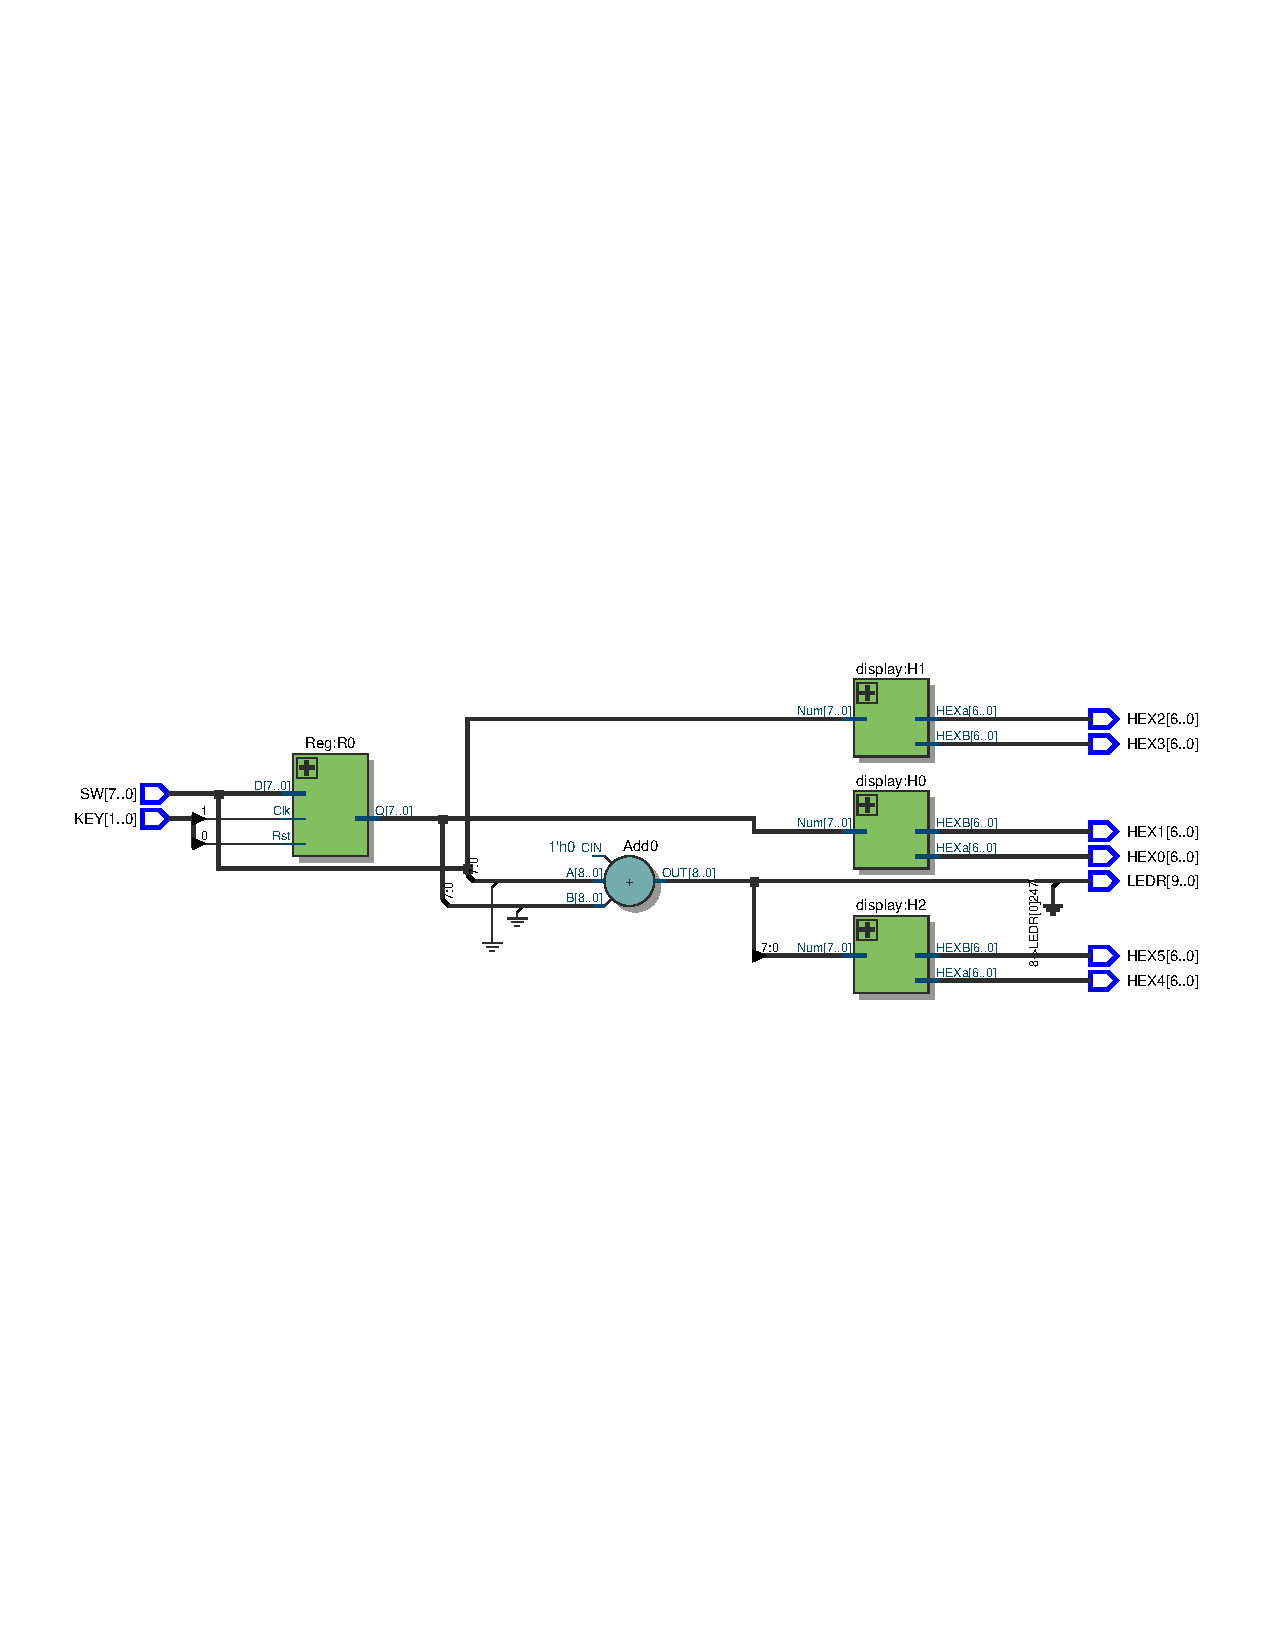
\includegraphics[width=1\textwidth]{Figures/Part5_RTL_TLE.jpg}
    \figcaption{RTL of the TLE}
    \label{fig:p5_RTL_TLE}
\end{figure}
\begin{figure}[h]
    \centering
    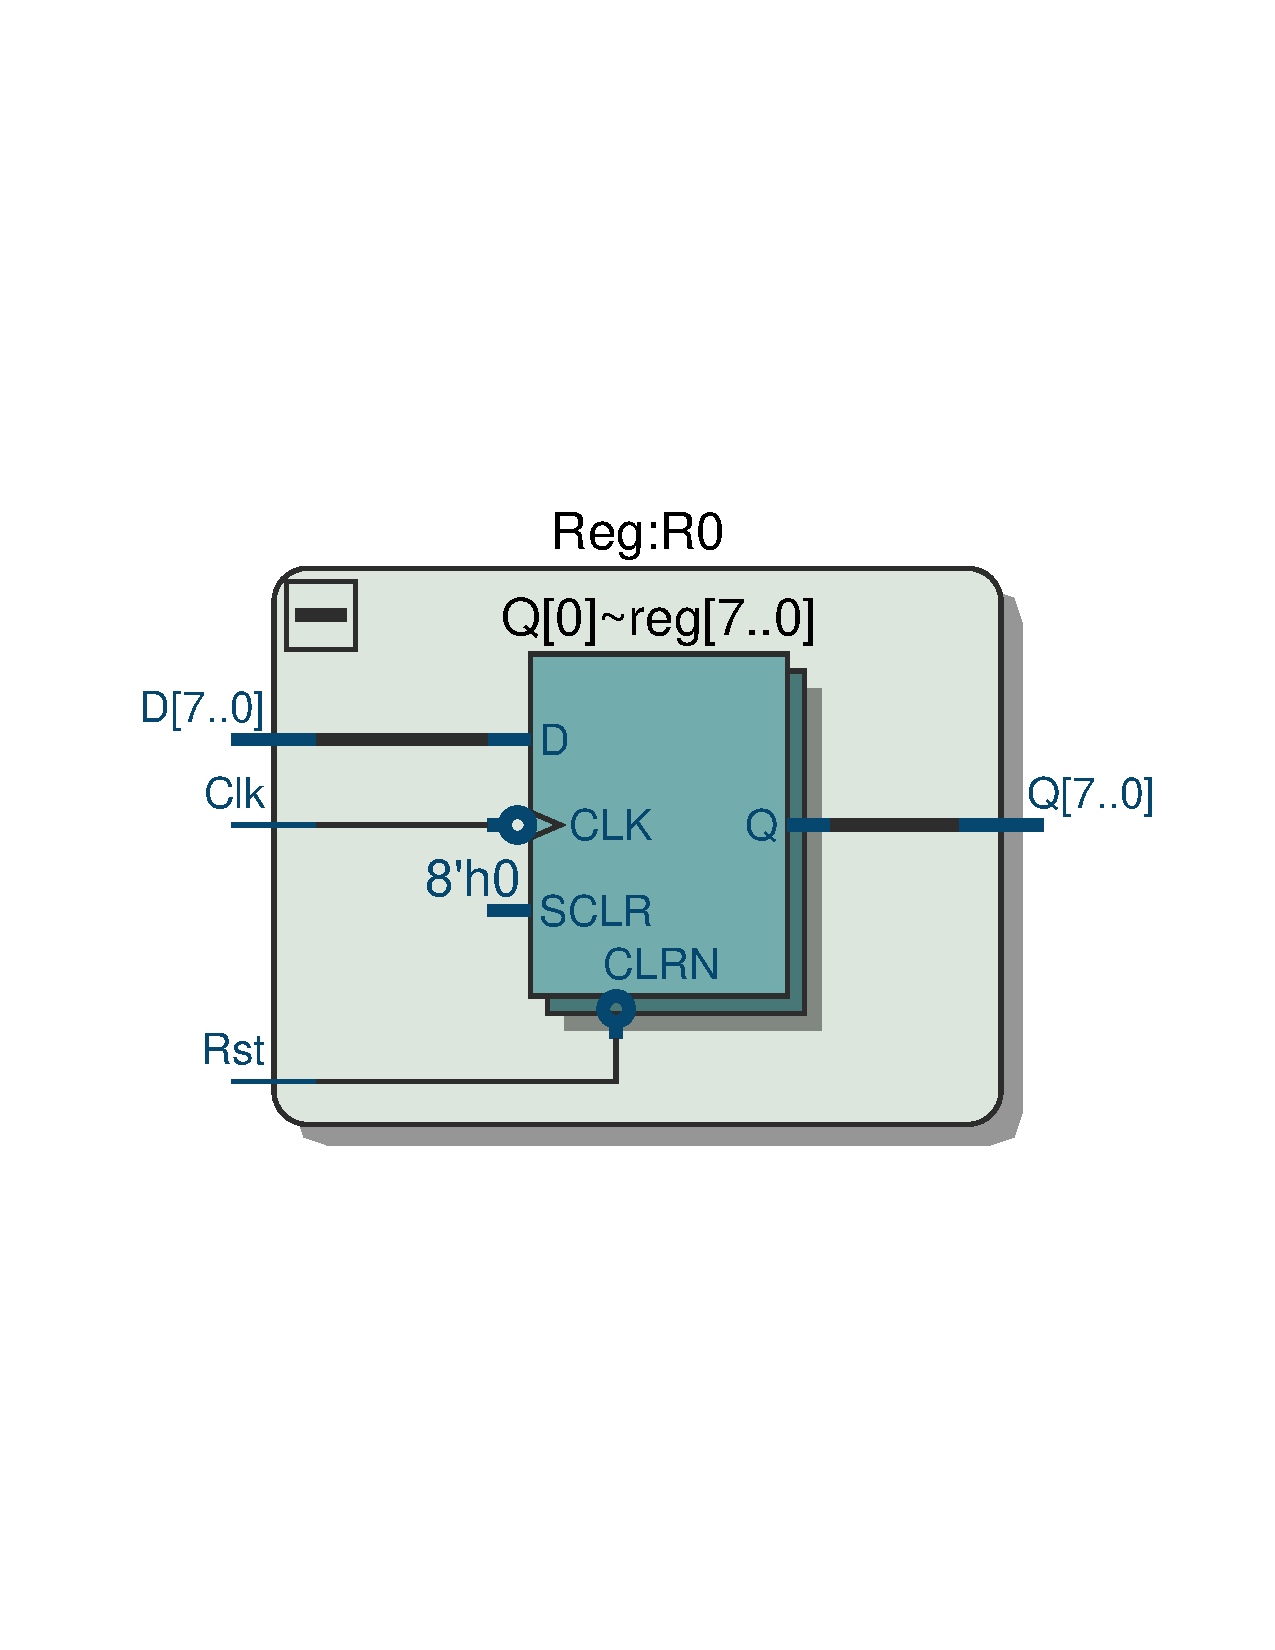
\includegraphics[width=0.6\textwidth]{Figures/Part5_RTL_Register.jpg}
    \figcaption{RTL of registry used in the TLE}
    \label{fig:p5_RTL_TLE}
\end{figure}
\clearpage
\begin{figure}[h]
    \centering
    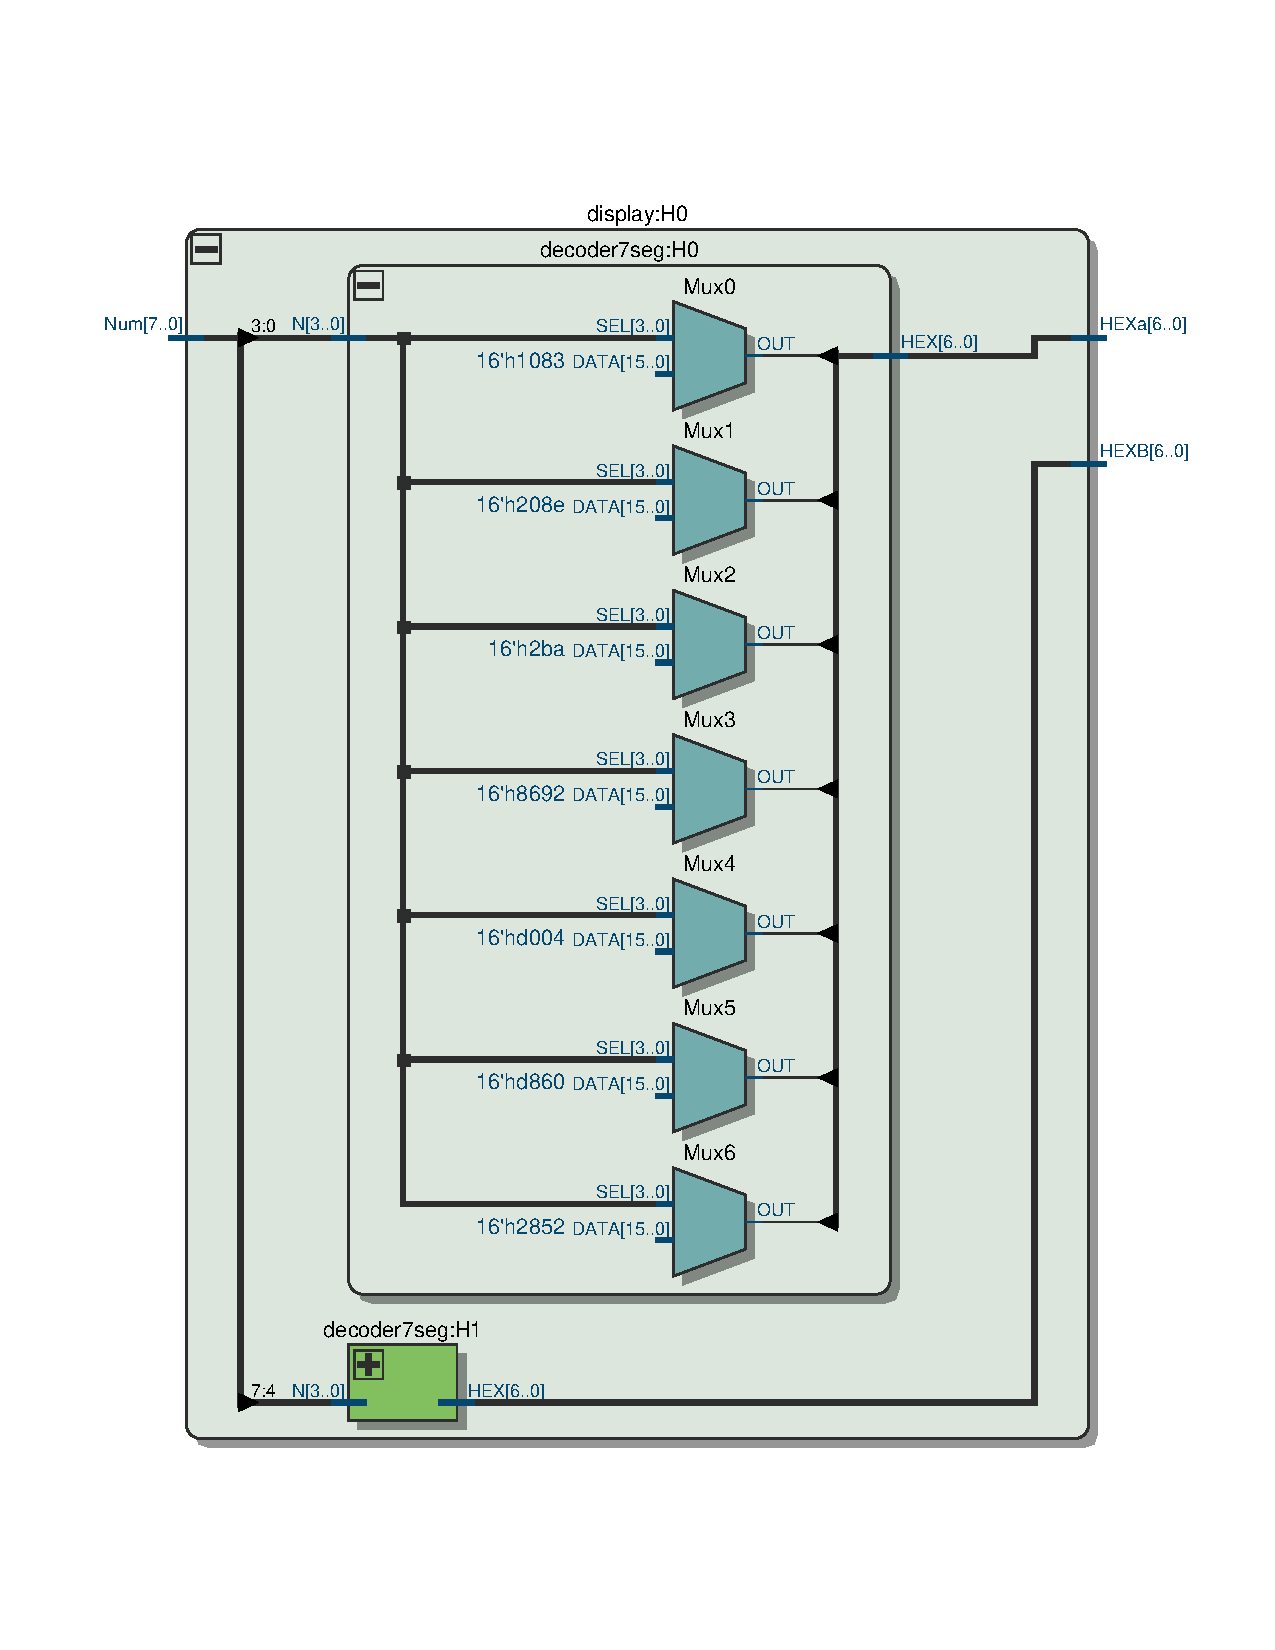
\includegraphics[width=1\textwidth]{Figures/Part5_RTL_Display.jpg}
    \figcaption{RTL of the Display component with two decoder instances}
    \label{fig:p5_RTL_TLE}
\end{figure}

\subsection{Results}
Implementing the code on the FPGA the results was as expected. The output is shown as the following: In \textcolor{red}{red}, the sum of \verb|A| and \verb|B|, in \textcolor{green}{green} the current switch value, \verb|A|, is show and in \textcolor{blue}{blue}, the stored number \verb|B|.

\clearpage
\begin{figure}[h]
    \centering
    \begin{subfigure}[t]{0.7\textwidth}
        \centering
        \includegraphics[width=1\textwidth]{Figures/Part5_1.jpg}
        \caption{00 = 00 + 00}
        \label{fig:p5_1}
    \end{subfigure}

    \begin{subfigure}[t]{0.7\textwidth}
        \centering
        \includegraphics[width=1\textwidth]{Figures/Part5_2.jpg}
        \caption{05 = 05 + 00}
        \label{fig:p5_2}
    \end{subfigure}
    
    \begin{subfigure}[t]{0.7\textwidth}
        \centering
        \includegraphics[width=1\textwidth]{Figures/Part5_3.jpg}
        \caption{0A = 05 + 05, Clk falling}
        \label{fig:p5_3}
    \end{subfigure}

    \begin{subfigure}[t]{0.7\textwidth}
        \centering
        \includegraphics[width=1\textwidth]{Figures/Part5_4.jpg}
        \caption{74 = BF + 05}
        \label{fig:p5_4}
    \end{subfigure}
    \figcaption{Results of part 5}
    \label{fig:p5_results}
\end{figure}

\begin{figure}[h]\ContinuedFloat
    \centering
    \begin{subfigure}[t]{0.7\textwidth}
        \centering
        \includegraphics[width=1\textwidth]{Figures/Part5_5.jpg}
        \caption{DE = BF + BF, Clk falling}
        \label{fig:p5_5}
    \end{subfigure}

    \begin{subfigure}[t]{0.7\textwidth}
        \centering
        \includegraphics[width=1\textwidth]{Figures/Part5_6.jpg}
        \caption{BE = FF + BF (overflow)}
        \label{fig:p5_6}
    \end{subfigure}
    
    \begin{subfigure}[t]{0.7\textwidth}
        \centering
        \includegraphics[width=1\textwidth]{Figures/Part5_7.jpg}
        \caption{FE = FF + FF (overflow), Clk falling}
        \label{fig:p5_7}
    \end{subfigure}

    \begin{subfigure}[t]{0.7\textwidth}
        \centering
        \includegraphics[width=1\textwidth]{Figures/Part5_8.jpg}
        \caption{FF = FF + 00, Reset falling}
        \label{fig:p5_8}
    \end{subfigure}
    \caption[]{Results of part 5 (continued)}
\end{figure}

\end{document}
